\documentclass[11pt,toc=sectionentrywithoutdots, 
headheight=44pt, headings=optiontoheadandtoc, hyperfootnotes=false]{scrartcl}

%Packages
\usepackage{geometry}

\geometry{
a4paper, 
left=30mm, 
right=25mm, 
top=25mm, 
bottom=25mm, 
headsep=5mm, 
footnotesep=5mm,
headheight=20mm,
footskip=15mm,
marginparwidth=15mm
}

\usepackage[utf8]{inputenc}
\usepackage{csquotes}
\usepackage{times}
\usepackage{verbatim}
\usepackage[T1]{fontenc}
\usepackage[ngerman]{babel}
\usepackage{graphicx}
\usepackage[headsepline]{scrlayer-scrpage}
\usepackage{blindtext}
\usepackage{footnotebackref}
\usepackage{nameref}
\usepackage{setspace}
\usepackage[automake]{glossaries}



\setstretch{1.2}

\usepackage[
backend=biber,
style=authortitle,
citestyle=authoryear
]{biblatex}

\addbibresource{literatur.bib}

 \usepackage{tikz,ifthen,xstring,calc,pgfkeys,pgfopts}
 \usepackage{tikz-uml}
 \usetikzlibrary{external}
 \tikzexternalize[prefix=figures/] % activate and define figures/ as cache folder

\usepackage{hyperref}
\usepackage[printonlyused, withpage]{acronym}

%%%%%%%%%%%%%%%%%% Compile optimization - Kill for release!!!%%%%%%%%%%%%%%
% Kill draft in Dokumentclass!!!
%\pdfcompresslevel=0
%\pdfobjcompresslevel=0
%%%%%%%%%%%%%%%%%%%%%%%%%%%%%%%%%%%%%%%%%%%%%%%%%%%%%%%%%%%%%%%%%%%%%%%%

\hypersetup{
    colorlinks=true,
    linktoc=page,
    linkcolor=blue,
    filecolor=magenta,      
    urlcolor=blue,
    citecolor=blue
}



%%%%%%%%%%%%%% Set line Spacing for Abbreviation %%%%%%%%%%%%%%%%%%
%\renewenvironment{description}
%{\list{}{\labelwidth0pt\itemindent-\leftmargin
%    \parsep0pt\itemsep0pt\let\makelabel\descriptionlabel}}
%               {\endlist}
%%%%%%%%%%%%%%%%%%%%%%%%%%%%%%%%%%%%%%%%%%%%%%%%%%%%%%%%%%%%%%%%%%%%%%

%\usetikzlibrary{external}
%\tikzexternalize %

%Function for getting sectionName---------------------------------------------------

\newcounter{secautolabel}
\AddtoDoHook{heading/endgroup}{\setautolabel}
\newcommand*{\setautolabel}[1]{%
  \stepcounter{secautolabel}%
  \label{sec:autolabel:\thesecautolabel}%
  \expandafter\xdef\csname #1title\endcsname{%
    \noexpand\nameref*{sec:autolabel:\thesecautolabel}%
  }%
}

\newcommand\sectionRefs{%
	\sectiontitle  
}


%Function for getting sectionName----------------------------------------------------



%Images path
\graphicspath{{./src/images/}}

%Document meta data
\geometry{bottom=25mm, right=25mm, left=25mm, top=35mm}

%Set page numbering font
\renewcommand{\headfont}{\normalfont}

\makeglossaries

\newglossaryentry{Query}
{
	name=Query,
	description={Datenbankanweisung, welche an einen Datenbankserver 		verschickt wird und dazu dient, Daten abzufragen, zu erstellen, zu verändern oder zu löschen}
}
\newglossaryentry{Assembly}
{
	name=Assembly,
	description={Logische Organisationseinheit in .NET, welche einen Baustein einer größeren Anwendung darstellt. Auch \glqq Komponente\grqq oder \glqq Modul\grqq genannt}
}
\newglossaryentry{Persistenz}
{
	name=Persistenz,
	description={Die theoretische Möglichkeit eines Objekts unendlich und unabhängig von der Software, in der es erzeugt wurde, zu existieren. In der Praxis kann keine hundertprozentige Persistenz gewährleistet werden}
}
\newglossaryentry{Customer Obsession}
{
	name=Customer Obsession,
	description={Wirtschaftsphilosophie, die den Kunden als Maßstab für alle Überlegungen des ökonomischen Denken und Handels emporhebt. Gemäß dieses Ansatzes gibt es keine den Wünschen des Kunden übergeordneten Maxime}
}
\newglossaryentry{Kanban}
{
	name=Kanban,
	description={Prinzip für das Abarbeiten von Aufgaben im Team, bei dem alle anfallenden Aufgaben mit einer Karte visualisiert werden, die in Säulen von festgelegter maximaler Stückzahl abgelegt sind. Steigt eine Aufgabe im Bearbeitungsstadium auf, wird sie von links nach rechts \glqq gepullt\grqq. Die rechteste Säule trägt immer den Namen \glqq Done\grqq}
}
\newglossaryentry{Product Owner}
{
	name=Product Owner,
	description={\glqq Der:die Product Owner:in ist ergebnisverantwortlich für die Maximierung des Wertes des Produkts, der
sich aus der Arbeit des Scrum Teams ergibt. Wie dies geschieht, kann je nach Organisation, Scrum Team
und Individuum sehr unterschiedlich sein\grqq\footnote{Entnommen aus \cite{SchwaberSutherland2020}} 
}
}


 
 
 
\begin{document}



\thispagestyle{empty}
\cfoot[]{}
%\ofoot{Seite \thepage\:von \pageref{LastPage}}
\ofoot{\thepage}
\ifoot{© Frank Loleit}
\ohead{
\includegraphics[scale=0.125]{argusLogo}}



\ihead
{%	
	\begin{small}
	
	
		MODUL FÜR GEKAPSELTE DATENBANKKOMMUNIKATION%		
		\newline\
		\textit\sectionRefs
	\end{small}%
}


%IHK-Logo
\begin{figure}[h]

\includegraphics[scale=0.25]{ihkLogo}
\centering
\end{figure}

\begin{center}
\begin{Large}

Abschlussprüfung Winter 2021
\linebreak

Fachinformatiker (Anwendungsentwicklung)\linebreak
Dokumentation der betrieblichen Projektarbeit
\linebreak\linebreak
\end{Large}


\begin{LARGE}
\begin{bfseries}
	Entwicklung eines Moduls in einer Desktopanwendung zur Umstellung von direkten Datenbankzugriffen zu einer gekapselten Datenbankkommunikation mit optionaler Simulationsmöglichkeit.
\linebreak\linebreak
\end{bfseries}
\end{LARGE}

\begin{Large}
%Backend-Applikation zur algorithmusbasierten 
%Erfassung von\linebreak Meldungen in sozialen Netzwerken
%\linebreak

Abgabetermin: 22.11.2021
\linebreak\linebreak
\begin{bfseries}
Auszubildender:\linebreak
\end{bfseries}
Frank Loleit\linebreak
Wildenbruchstr. 43\linebreak
12435 Berlin\linebreak

\begin{figure}[h]

\includegraphics[scale=0.25]{argusLogo}
\centering
\end{figure}



\begin{bfseries}
Ausbildungsbetrieb:\linebreak
\end{bfseries}
ARGUS DATA INSIGHTS® Deutschland GmbH\linebreak
Gneisenaustr. 66\linebreak
10961 Berlin


\end{Large}


\end{center}





\newpage
\setcounter{page}{1}
\pagenumbering{Roman}


\tableofcontents


\setcounter{secnumdepth}{0}

\newpage

\phantomsection
\addcontentsline{toc}{section}{Abbildungsverzeichnis}
\listoffigures




\newpage

\phantomsection
\addcontentsline{toc}{section}{Tabellenverzeichnis}
\listoftables
\newpage

%\section{Listings}
%\blindtext\blindtext\blindtext
%\newpage

\section{Abkürzungsverzeichnis}


\begin{acronym}[xxxxxxx]

\acro{ADI}{Argus Data Insights Deutschland GmbH}
\acro{CRUD}{Create, Read, Update, Delete}
\acro{GUI}{Graphical User Interface}
\acro{XAML}{Extensible Application Markup Language}
\acro{DRY}{Don't Repeat Yourself}
\acro{SQL} {Structured Query Language}
\acro{SSMS} {SQL Server Management Studio}

\end{acronym}
\newpage

\phantomsection
\addcontentsline{toc}{section}{Glossar}
\printglossary[nonumberlist]
\newpage


\setcounter{secnumdepth}{1}
\pagenumbering{arabic}
\setcounter{secnumdepth}{4}
\ofoot{Seite\:\thepage}%\:von \pageref*{myLastPage}%}

\section{Einleitung}
In diesem Projekt wird das Ziel verfolgt, die Datenbankkommunikation einer Desktopanwendung zu vereinheitlichen und die Arbeit der Entwickler von der Arbeit der Nutzer abzugrenzen. Obgleich es sich bei dem entwickelten Modul um ein Werkzeug handelt, das nur von Entwicklern geöffnet und verwendet werden kann, steht der Kunde im Vordergrund aller Bemühungen. Denn sowohl das Auffinden und Lösen von Programmfehlern, wie auch das Implementieren von neuen Komponenten kann durch die Vereinheitlichung und Separierung der Datenbankoperationen deutlich effizienter werden. Der Kunde erhält dadurch nicht nur ein tendenziell stabileres System, sondern kann auch damit rechnen, dass neue gewünschte Funktionalitäten schneller umgesetzt werden. In diesem Sinne steht bei allen Bemühumgen dieses Projektes stets die \gls{Customer Obsession} im Vordergrund.

\subsection{Projektbeschreibung}
Ausgangspunkt der Arbeit ist die Desktopapplikation \glqq Arche\grqq{}, entwickelt im .NET-Framework\footnote{\cite{Microsoft2020}} 3.5 mit WinForms-\acs{GUI}. Das Debugging gestaltet sich teils als recht aufwändig, da alle Funktionen umgangen werden müssen, die Kundendaten generieren, verändern oder löschen. Grund dafür ist das Fehlen von Mechanismen, durch die sich Datenbankoperationen, die von Kunden und Entwicklern vorgenommen werden, jeweils voneinander abgrenzen lassen. Auch das Implementieren von neuen datenbanksensiblen Features gestaltet sich als umständlich, da es kein einheitliches Prinzip für die Datenbankkommunikation gibt. Viel mehr hat jeder einzelne Workflow jeweils eine eigene Klasse für die Datenbankkommunikation, die sich inhaltlich aber kaum unterscheiden, sondern im Wesentlichen voneinander kopiert wurden und das \acs{DRY}-Prinzip wenig Berücksichtigung findet. Daher soll ein Modul entwickelt werden, dass die Kommunikation mit der Datenbank kapselt.\newline Zunächst soll es möglich sein, dass eine \gls{Query}, die ein beliebiger Workflow an den Datenbankserver übergibt, zurückgehalten werden kann und somit nicht Gefahr zu laufen, unerwünschte Änderungen an Datenbankeinträgen vorzunehmen. Dabei soll in einer für Entwickler bestimmten GUI die entsprechende Query mit sinnvoller Hervorhebung entsprechender Keywords erfolgen. Zudem soll der Entwickler frei entscheiden können, ob die Query verarbeitet, zurückgehalten oder in ein \acs{SQL}-Management-System übertragen werden soll. Im Anschluss soll die uneinheitliche Datenbankkommuniktation durch eine globale Logik mit Hilfe von Datenbankmodellen ersetzt werden. Aus diesen Modellen soll schlussendlich ein einheitliches Verfahren abgeleitet werden können, das die Datenbankanbindung auf ein einziges \gls{Assembly} des Projektes konzentriert und somit eine langfristige Arbeitserleichterung schafft.

\subsection{Projektziel}
Nach Abschluss des Projektes muss es möglich sein, in Arche Insert-, Update- und Delete-Funktionen auszulösen, ohne dabei Kundendaten zu beeinträchtigen. Ist das zu entwickelnde Modul aktiv und es wird in der GUI von Arche ein Speichern- oder Löschen-Button geklickt, soll Arche angehalten und stattdessen ein Fenster öffnen, das nur für Entwickler bestimmt ist. Dieses gibt nun die Query aus, welche an den Datenbankserver geschickt worden wäre. Die Möglichkeit, die Query mit einem Klick umgehend nach \acs{SSMS} zu versenden muss ebenfalls gegeben sein, wie die Funktion, frei entscheiden zu könnnen, ob die Query von Arche ausgeführt wird oder nicht. Die Entwickler müssen die Möglichkeit erhalten die Datenbank lokal zu simulieren und die entsprechenden Queries lokal auszuführen. Zudem muss ein einheitliches auf Datenbankmodellen basierendes Prinzip implementiert werden, über welches jedwede Insert-, Update- und Delete-Query mit entsprechenden Parametern generiert werden kann.%keine Unstimmigkeiten mit dem 
%Webinterface auftreten. Die \acs{ADI} ist daher bemüht weitere Schritte %einzuleiten. Man hat sich entschieden \acs{XAML} zu verwenden. Auch %Mathematisch ist dies wichtig\footnote{vgl. \cite{GeraldTeschl2008}}.

\subsection{Projektumfeld}
Argus Data Insights (im Folgenden \glqq Argus\grqq{} genannt) ist darauf spezialisiert, Print- , Video- und Onlinemedien - insbesondere Zeitungen, Fernsehen und soziale Netzwerke - für angefragte Zeiträume und Themen zu durchsuchen und dem Kunden skalierbare Dossiers mit Informationen zur eigenen Person, Firma oder Einrichtung zu geben. Die Kunden erlangen auf diese Weise einen detaillierten Einblick darüber, wie viel Aufmerksamkeit der Kunde in den Medien allgemein erhält, welche Themen mit dem Kunden assoziiert werden und und die Berichterstattung tendenziell positiv, negativ oder neutral ausfällt. Die Redaktionssoftware Arche wird sowohl zum Digitalisieren, Annotieren, Aufbereiten und Versenden der für den Kunden angefertigten Dossiers verwendet. Dabei werden vor allem Print- und Onlineinhalte unterschieden. Die verschiedenen Medieninhalte werden in Fileservern abgelegt, deren Pfade sowie zahlreiche Medienparameter in Datenbanktabellen gespeichert. Darüber hinaus gibt es eine umfangreiche Kundendatenbank. Datenbankzugriffe erfolgen nicht einheitlich, sondern von verschiedenen \gls{Persistenz}-Klassen aus, deren interne Logik von jeweils der zuletzt angelegten Persistenzklasse kopiert ist (nicht vererbt).

\subsection{Projektbegründung}
Die Gründe für das Projekt liegen in der erschwerten Wartung der Software, sowie dem erhöhten Aufwand, neue datenbanksensible Komponenten hinzuzufügen. Muss ein Ticket\footnote{Bei Argus wird das \gls{Kanban}-Board \href{https://www.atlassian.com/software/jira}{Atlassian Jira} verwendet.} bearbeitet werden, bei dem ein Problem mit Query und oder Datenbank vermutet wird, müssen beim Debugging sehr früh Breakpoints gesetzt werden, um nicht Gefahr zu laufen, Kundendaten irreversibel zu verändern. Es fehlt die Möglichkeit, global die Ausführung von Datenbankprozessen zurückzuhalten. Darüber hinaus ist es äußerst kompliziert, die entsprechende Query zu erhalten, welche es für das jeweilige Ticket zu analysieren gilt. Daran anschließend ist kein einheitlicher Prozess vorhanden, der die Kommunikation von .NET und MSSQL steuert. Um sowohl Wartbarkeit, als auch einfache Erweiterbarkeit zu gewährleisten, ist dieses Projekt in Absprache mit den \gls{Product Owner}n entstanden.

\subsection{Projektabgrenzung}
Durch die komponentenorientierte Arbeitsweise in .NET lässt sich das zu entwickelnde Modul gut von bereits fertigen Projekten innerhalb der Kernapplikation Arche abgrenzen \autoref{fig:Assemblies}

\section{Projektplanung}
Eine sinnvolle Planung für das Projekt ist natürlich wichtig. Aber man sollte es auch nicht übertreiben.

\subsection{Projektphasen}
Das Projekt wurde in einem Zeitraum von 70 Stunden umgesetzt. 
Dabei wurde die gesamte Stundenanzahl wurde wie folgt aufgeteilt:


\begin{table}[ht]
	\begin{center}
		\begin{tabular}{ ||l|r|| }
			\hline
			\textbf{Projektphase} 		& \textbf{Geplante Zeit} \\
			\hline

			Analysephase 				& 8 h	 		\\
			Entwurfsphase				& 11 h	 		\\
			Implementierungsphase 		& 40 h	 		\\
			Abnahme und Einführung		& 11 h 			\\
			Erstellen der Dokumentation & 10 h 			\\
			\hline
			\textbf{Gesamt}	 			& \textbf{70 h}	\\
			
			\hline
		\end{tabular}
		\caption{Zeitplanung}
	\end{center}
\end{table}	


\subsection{Ressourcenplanung}
\blindtext\

\subsection{Entwicklungsprozess}
\blindtext\

\section{Analysephase}
\blindtext\

\subsection{IST-Zustand}
Momentan kann Arche nur

\subsection{Wirtschaftlichkeitsanalyse}
\blindtext\

\subsubsection{Beschaffung der Ausgangsdaten}
\blindtext\

\subsubsection{Ermitteln der Kostenstruktur}
\blindtext\

\subsubsection{Kostenberechnung}
\blindtext\

\subsubsection{Zusammenstellen des Kostenplans}
\blindtext\

\subsubsection{Nicht-monetäre Vorteile}
\blindtext\

\subsection{Anwendungsfälle}
\blindtext\

\subsection{Lastenheft}
\blindtext\

\subsection{Risikomanagement}
\blindtext\

\subsubsection{Risikoerkennung}
\blindtext\

\subsubsection{Risikoanalyse}
\blindtext\

\subsubsection{Risikominimierung}
\blindtext\

\section{Entwurfsphase}
\blindtext\

\subsection{Zielplattform}
\blindtext\

\subsection{Architekturdesign}
\blindtext\

\subsection{Entwurf des Datenmodells}
\blindtext\

\subsection{Entwurf Geschäftslogik}
\blindtext\

\subsubsection{Entwurf Geschäftslogik}
\blindtext\

\subsubsection{Entwurf Modul Extraktion}
\blindtext\

\subsubsection{Entwurf Modul Laden}
\blindtext\

\subsubsection{Entwurf Modul Transformation}
\blindtext\

\subsection{Roundtrip Engineering}
\blindtext\

\subsection{Pflichtenheft}
\blindtext\

\section{Implementierung}
\blindtext\

\subsection{Implementierung Extraktion}
\blindtext\

\subsection{Implementierung Laden}
\blindtext\

\subsection{Implementierung der Datenstrukturen}
\blindtext\

\subsection{Implementierung Transformation}
\blindtext\

\subsection{Implementierung Hilfsklassen und Interfaces}
\blindtext\

\section{Qualitätssicherung}
\blindtext\

\subsection{Systemtest}
\blindtext\

\subsection{Tests gegen das System}
\blindtext\

\subsection{Testprotokolle}
\blindtext\

\section{Abnahme}
\blindtext\

\subsection{Soll/Ist-Vergleich}
\blindtext\

\subsection{Abnahme durch den technischen Leiter}
\blindtext\

\section{Dokumentation}
\blindtext\

\subsection{Technische Dokumentation}
\blindtext\

\subsection{Nutzerdokumentation}
\blindtext\

\section{Fazit}
\blindtext\

\subsection{Im Laufe des Projektes gewonnene Erkenntnisse}
\blindtext\

\subsection{Ausblick}
\blindtext\

\subsubsection{Von Anfang an geplante Weiterentwicklung}
\blindtext\

\subsubsection{Im Laufe des Projektes erkannter Weiterentwicklungsbedarf}
\blindtext\


\newpage
\setcounter{secnumdepth}{0}

\phantomsection
\addcontentsline{toc}{section}{Literatur}

\printbibliography



\label{myLastPage}

\newpage

\pagenumbering{roman}

\setcounter{page}{1}
\setcounter{secnumdepth}{2}
\setcounter{section}{1}
\renewcommand{\thesection}{A}


\ofoot{\thepage}



\section{Anhang}

\subsection{Detaillierte Zeitplanung}

\begin{table}[ht]
	\begin{center}
		\begin{tabular}{ ||l|r|| }
			\hline
			
			\textbf{Analysephase} 										& \textbf{8 h}	\\
			\hline			
			1. Ist-Analyse												& 5 h			\\
			2. Wirtschaftlichkeitsprüfung								& 2 h			\\		
			3. Kommunikation mit dem Fachbereich						& 1 h			\\
			\hline

			\textbf{Entwurfphase} 										& \textbf{11 h}	\\
			\hline
			1. Frameworks auswählen										& 1 h			\\
			2. Projektbesprechung mit Tutoren							& 2 h			\\		
			3. Graphische Benutzeroberfläche skizzieren					& 2 h			\\
			4. Datenbankmodell entwerfen								& 3 h			\\
			5. Geschäftslogik ausformulieren							& 3 h			\\			
			\hline

			\textbf{Implementierungsphase} 								& \textbf{40 h}	\\
			\hline
			1. Datenbank aufsetzen										& 11 h 			\\
			2. Modelle einpflegen und testen							& 11 h 			\\
			3. Komponenten erstellen 									& 11 h 			\\
			4. ViewModels programmieren	und an GUI andocken				& 11 h 			\\
			5. Controller anlegen										& 11 h 			\\
			6.1 Python-Skripte einpflegen								& 11 h 			\\
			6.2 C\# Properties anlegen									& 11 h 			\\
			6.3 Debuggen												& 11 h 			\\
			6.4 Tests ausführen											& 11 h 			\\
			6.4 Pull Requests bearbeiten								& 11 h 			\\			
			\hline

			\textbf{Abnahme und Schulung}		 						& \textbf{2 h}	\\
			\hline
			1. Abnahme durch Fachabteilung								& 11 h 			\\
			2. Installation												& 11 h 			\\
			\hline

			\textbf{Erstellen der Dokumentation} 						& \textbf{10 h}	\\
			\hline
			1. Erstellen der Projektdokumentation						& 11 h 			\\
			2. Erstellen der Entwicklerdokumentation					& 11 h 			\\
			3. Erstellen Benutzerdokumentation							& 11 h 			\\
			\hline

			\textbf{Gesamt}	 											& \textbf{70 h}	\\
			\hline

		\end{tabular}
		%\caption{Zeitplanung}
	\end{center}
\end{table}	

\subsection{Ressourcenplan}
\blindtext\blindtext

%\subsection{Projektkosten Details}
%\blindtext\blindtext
\subsection{Auszüge Assemblies}
Einige Komponenten aus Arche mit den Komponenten DBEncapsulation und DBEncapsulationTests:
 \begin{figure}[h]
 \centering



 \label{fig:Assemblies}
	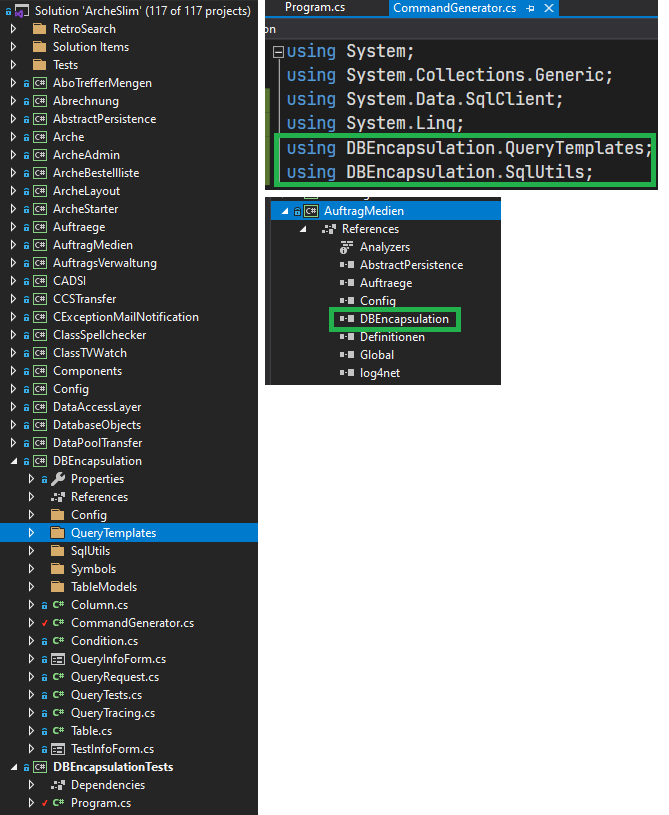
\includegraphics[scale=0.7]{Assemblies.png}
	 \caption{Assemblies}
 \end{figure}


\subsection{Anwendungsfalldiagramm}
\blindtext\blindtext

\subsection{Lastenheft (Auszug)}
\blindtext\blindtext

\subsection{Quell- und Zieldatenschema}
\blindtext\blindtext

\subsection{Sequenzdiagramm}
\blindtext


\subsection{Klassendiagramm}

Dies ist ein Beispiel für ein UML-Klassendiagramm:\\

 \begin{figure}[ht]
 \centering
 \begin{tikzpicture}

 	\umlclass[x=5, y= 0]{Person}	
 		{
 			- vorerkrankungen : String\\
 			- religion : string\\
 			+ alter : int\\
 			+ name : String\\
 			+ geschlecht : String\\
			
 		}
 		{
 			+ halloSagen() : void		\\	
 			+ freundlichLaecheln() : void		\\	
 		}
		
		
 	\umlclass[x=0, y= -6]{Kind}	
 		{
 			- kinderGarten: String\\
 			+ hobbys : String \\
 			+ magNutella : bool \\
 		}
 		{
 			- inDieSchuleGehen() : void	\\
 			- dreiradFahren() : void\\
 			+ getKindergarten() : String\\
			
 		}	
		
		
 	\umlclass[x=10, y= -6]{Erwachsener}	
 		{
 			- beruf: String\\
 			- kontostand : double\\
 			+ hatKinder : bool\\
 		}
 		{
 			- zurArbeitGehen() : void	\\
 			- autoFahren() : void\\
 			+ getBeruf() : String\\
			
 		}
		
 		\umlnote{Person}{Dies ist offensichtlich eine Klasse}		
 		\umlinherit[geometry=|-]{Erwachsener}{Person}
 		\umlinherit[geometry=-|]{Kind}{Person}
 		\umldep[very thick, arg1=0..*, arg2=1..*, pos1=0.05, pos2=0.52,anchor1=-20, anchor2=-20]{Kind}{Erwachsener}

	
 \end{tikzpicture}

 \caption{Klassendiagramm}
 \label{fig:Klassendiagramm}
	
 \end{figure}

\subsection{Pflichtenheft (Auszug)}
Dies ist ein bisschen Text

\subsection{Laufzeitdiagnose}
\blindtext

\subsection{Ganttdiagramm}
\blindtext

\subsection{Projektstrukturplan}
\blindtext

\subsection{Arbeitspakete}
\blindtext

\subsection{Arbeitspaketressourcen im Detail}
\blindtext

\end{document}